\documentclass{article}
\usepackage{graphicx}
\usepackage{amsmath}
\usepackage{pgfplots}
\usepackage{physics}
\usepackage{cancel}
\usepackage{enumitem}
\usepackage{txfonts}

\newcommand{\g}{\text{g}}
\newcommand{\kilo}{\text{k}}
\newcommand{\m}{\text{m}}
\newcommand{\centi}{\text{c}}
\newcommand{\s}{\text{s}}
\newcommand{\N}{\text{N}}
\newcommand{\J}{\text{J}}
\newcommand{\C}{\text{C}}
\newcommand{\V}{\text{V}}
\newcommand{\A}{\text{A}}
\newcommand{\Ohm}{\text{\Omega}}

\pgfplotsset{compat=1.18}

\usepackage[a4paper, top=1cm, bottom=2cm, left=2cm, right=2cm, includehead, includefoot]{geometry}

\begin{document}

\noindent
Physics 4B - Electromagnetism \hfill Prof. Alfred Cauthen

\noindent\rule{\textwidth}{0.4pt}

\begin{center}
    \textbf{\LARGE Homework 6} \\
    \vspace{12pt}
    \large Aaron W. Tarajos \\
    \textit{\today}
\end{center}

\noindent\rule{\textwidth}{0.4pt}

\section*{Chapter 23 Question 1}
A surface has the area vector $\vec A = (2\vu i + 3\vu j)\ \m^2$. What is the flux of a uniform electric field through the area if the field is (a) $\vec E = 4\vu i$ N/C and (b) $\vec E = 4\vu k$ N/C?

\subsection*{Solution}
The flux through the surface is given from an electric field $\vec{E}$ and a surface $\vec{A}$ by;
\begin{equation*}
    \Phi_E = \vec{E} \cdot \vec{A}
\end{equation*}
so we have
\begin{enumerate}[label=(\alph*)]
    \item 
        \begin{equation*}
            \Phi_E = \vec{E} \cdot \vec{A} = 4\vu i \cdot (2\vu i + 3\vu j) = 8\ \frac{\N\m^2}{\C}
        \end{equation*}
    \item 
        \begin{equation*}
            \Phi_E = \vec{E} \cdot \vec{A} = 4\vu k \cdot (2\vu i + 3\vu j) = 0\ \frac{\N\m^2}{\C}
        \end{equation*}
\end{enumerate}

\section*{Chapter 23 Question 3}
Figure 23-23 shows, in cross section, a central metal ball, two spherical metal shells, and three spherical Gaussian surfaces of radii $R$, $2R$, and $3R$, all with the same center. The uniform charges on the three objects are: ball, $Q$; smaller shell, $3Q$; larger shell, $5Q$. Rank the Gaussian surfaces according to the magnitude of the electric field at any point on the surface, greatest first.

\begin{figure}[ht]
    \centering
    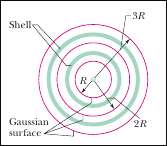
\includegraphics[scale=0.75]{image.png}
\end{figure}

\subsection*{Solution}
The electric field of all 3 Gaussian surfaces are the same. For a given surface the electric field is given by;
\begin{align*}
    \vec{E} &= \frac{Q}{4\pi \varepsilon_0 r^2} \vu r
\end{align*}
so now we adjust $Q$ and $r$ for the respective surfaces;
\begin{align*}
    \vec{E}_1 &= \frac{Q}{4\pi \varepsilon_0 R^2} \vu r \\
    \vec{E}_2 &= \frac{4Q}{4\pi \varepsilon_0 (2R)^2} \vu r  = \frac{Q}{4\pi \varepsilon_0 R^2} \vu r \\
    \vec{E}_3 &= \frac{9Q}{4\pi \varepsilon_0 (3R)^2} \vu r = \frac{Q}{4\pi \varepsilon_0 R^2} \vu r
\end{align*}
therefore, all 3 fields are equal.

\section*{Chapter 23 Question 6}
Three infinite nonconducting sheets, with uniform positive surface charge densities $\sigma$, $2\sigma$, and $3\sigma$, are arranged to be parallel like the two sheets in Fig. 23-19a. What is their order, from left to right, if the electric field $E$ produced by the arrangement has magnitude $E = 0$ in one region and $E = 2\sigma/\varepsilon_0$ in another region?

\subsection*{Solution}
The order would be $3\sigma$, $1\sigma$, $2\sigma$ because the the electric field from one side of a single sheet of charge density $\sigma$ is given by;
\begin{align*}
    \Phi &= \vec{E} \cdot \vec{A} \\
	\vec{E} \cdot \vec{A} &= \frac{Q_\text{enc}}{\varepsilon_0} \\
    \vec{E} \cdot \vec{A} &= \frac{\sigma \vec{A}}{\varepsilon_0} \\
    \vec{E} &= \frac{\sigma}{\varepsilon_0}
\end{align*}
assume that the direction orthogonal to the surface is the $z$ direction, then the electric field in the first region is;
\begin{equation*}
    \vec{E} = \frac{3\sigma}{\varepsilon_0} \vu z - \frac{\sigma}{\varepsilon_0} \vu z - \frac{2\sigma}{\varepsilon_0} \vu z = 0
\end{equation*}
and the electric field in the second region is;
\begin{equation*}
    \vec{E} = \frac{3\sigma}{\varepsilon_0} \vu z + \frac{\sigma}{\varepsilon_0} \vu z - \frac{2\sigma}{\varepsilon_0} \vu z = \frac{2\sigma}{\varepsilon_0} \vu z
\end{equation*}

\section*{Chapter 23 Question 8}
Figure 23-27 shows four solid spheres, each with charge $Q$ uniformly distributed through its volume. (a) Rank the spheres according to their volume charge density, greatest first. The figure also shows a point $P$ for each sphere, all at the same distance from the center of the sphere. (b) Rank the spheres according to the magnitude of the electric field they produce at point $P$, greatest first.

\begin{figure}[ht]
    \centering
    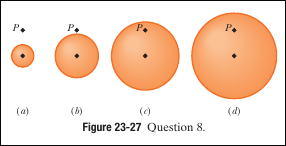
\includegraphics[scale=0.75]{image-2.png}
\end{figure}

\subsection*{Solution}
\textbf{Part a:} The ranked order by volume charge density is $a > b > c >$ because the less volume the sphere has the less space the charge is spread through making the density higher.\vspace{12pt}\\
\textbf{Part b:} We have two spheres with an internal point and two spheres with an external point. Using Gauss's law we can find the electric field for the spheres with an external point. Imagine a gaussian surface drawn through the point $P$ for each sphere. The electric field is given by;
\begin{align*}
    \vec{E} &= \frac{Q}{4\pi \varepsilon_0 r^2} \vu r
\end{align*}
the other sphere with the external point has the same electric field because the point $P$ is fixed and the charge within the Gaussian surface is the same. Now for the spheres with the internal point we use a similar idea, imagine a gaussian surface drawn around the point $P$ for each sphere. The electric field is given by;
\begin{align*}
    \vec{E} &= \frac{Q}{4\pi \varepsilon_0 r^2} \vu r
\end{align*}
except the value of $Q$ is different for the two spheres because they have different charge densities. It's clear that the sphere with the sphere with the smaller volume will have the higher charge density and therefore the highest electric field. The ranked order is $a = b > c > d$.

\section*{Chapter 23 Problem 10}
Figure 23-34 shows a closed Gaussian surface in the shape of a cube of edge length $2.00\ \m$. It lies in a region where the non-uniform electric field is given by $\vec E = (3.00x + 4.00)\vu i + 6.00\vu j + 7.00\vu k\ \N/\C$, with $x$ in meters. What is the net charge contained by the cube?

\begin{figure}[ht]
    \centering
    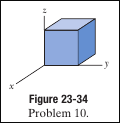
\includegraphics[scale=0.75]{image-3.png}
\end{figure}

\subsection*{Solution}
We start by calculating the flux through the cube.
\begin{align*}
    \Phi &= \oint \vec{E} \cdot d\vec{A} \\
    &= \int \nabla \vec{E} \cdot dV \\
    &= \int \left( \frac{\partial \vec{E}}{\partial x} + \frac{\partial \vec{E}}{\partial y} + \frac{\partial \vec{E}}{\partial z} \right) dV \\ 
    &= \int \left( 3.00 + 0 + 0 \right) dV \\
    &= \iiint 3\ dx\ dy\ dz \\
    &= 3L^3 \\
    &= 3 \cdot 2^3 \\
    &= 24
\end{align*}
and the charge enclosed by the cube is given by;
\begin{align*}
    Q_\text{enc} &= \varepsilon_0 \Phi \\
    &= \varepsilon_0 \cdot 24 \\
    &= 8.85 \times 10^{-12} \cdot 24 \\
    &= \boxed{2.12 \times 10^{-10} \C}
\end{align*}
because of the chapter content this was obviously supposed to be done by summing the flux through each face of the cube, but I just thought this was easier to show rigorously.

\section*{Chapter 23 Problem 12}
Figure 23-36 shows two non-conducting spherical shells fixed in place. Shell 1 has uniform surface charge density $+6.0\ \mu\C/\m^2$ on its outer surface and radius $3.0\ \centi \m$; shell 2 has uniform surface charge density $+4.0\ \mu\C/\m^2$ on its outer surface and radius $2.0\ \centi \m$; the shell centers are separated by $L = 10\ \centi \m$. In unit-vector notation, what is the net electric field at $x = 2.0\ \centi \m$?

\begin{figure}[ht]
    \centering
    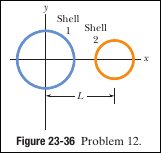
\includegraphics[scale=0.75]{image-4.png}
\end{figure}

\subsection*{Solution}
The net electric field inside of a shell charge is zero, so we only need to consider the electric field from shell 2.
\begin{align*}
    E &= \frac{Q}{4\pi \varepsilon_0 r^2} \\
    &= \frac{4\pi R^2 \sigma}{4\pi \varepsilon_0 r^2}\\
    &= \frac{R^2 \sigma}{\varepsilon_0 r^2} \\
    &= \frac{(2 \times 10^{-2})^2 (4 \times 10^{-6})}{(8.85 \times 10^{-12}) (8 \times 10^{-2})^2} \\
    &= \boxed{2.825 \times 10^4 \frac{\N}{\C}}
\end{align*}

\section*{Chapter 23 Problem 18}
The electric field just above the surface of the charged conducting drum of a photocopying machine has a magnitude $E$ of $2.3 \times 10^5\ \N/\C$. What is the surface charge density on the drum?

\subsection*{Solution}
The electric field is given by;
\[
    E = \frac{\sigma}{\varepsilon_0}
\]
so we have;
\begin{align*}
    \sigma &= \varepsilon_0 E \\
    &= 8.85 \times 10^{-12} \cdot 2.3 \times 10^5 \\
    &= \boxed{2.036 \times 10^{-6} \frac{\C}{\m^2}}
\end{align*}

\section*{Chapter 23 Problem 22}
An electron is released $9.0\ \centi \m$ from a very long nonconducting rod with a uniform $6.0\ \mu\C/\m$. What is the magnitude of the electron's initial acceleration?

\subsection*{Solution}
The field is given by;
\[
	E = \frac{\lambda}{2\pi \varepsilon r}
\]
and the force is just $q E$ so using Newton's second law
\begin{align*}
	a &= \frac{F}{m} \\
	&= \frac{q\lambda}{2\pi \varepsilon_0 r m} \\
	&= \frac{\left(1.602 \times 10.0^{-19}\right)\left(6.0 \times 10^{-6}\right)}{2\pi \varepsilon_0 (0.09)\left(9.109 \times 10^{-31}\right)} \\
	&= \boxed{2.108\times10^{17}\ \m/\s^2}
\end{align*}

\section*{Chapter 23 Problem 28}
A charge of uniform linear density $2.0\ \text{n}\C/\m$ is distributed along a long, thin, nonconducting rod. The rod is coaxial with a long conducting cylindrical shell (inner radius = $5.0\ \centi \m$, outer radius = $10\ \centi \m$). The net charge on the shell is zero. (a) What is the magnitude of the electric field $15\ \centi \m$ from the axis of the shell? What is the surface charge density on the (b) inner and (c) outer surface of the shell?

\subsection*{Solution}
\textbf{Part a:} We can use Gauss' law here;
\begin{align*}
    \vec{E} \cdot \vec{A} &= \frac{Q}{\varepsilon_0} \\
    \vec{E} \cdot 2\pi r L &= \frac{\lambda L}{\varepsilon_0} \\
    \vec{E} &= \frac{\lambda}{2\pi \varepsilon_0 r} \\
    &= \frac{2 \times 10^{-9}}{2\pi \varepsilon_0 0.15} \\
    &= \boxed{239.781 \frac{\N}{\C}}
\end{align*}
\textbf{Part b:} The linear charge density of the inside of the shell must be equal but opposite to the rod. We convert that to the surface charge density by
\begin{align*}
	\sigma &= \frac{-\lambda}{2\pi r} \\
		   &= \frac{-2.0 \times 10^{-9}}{2\pi 0.05} \\
		   &= \boxed{-6.366\ \times 10^9\ \C/\m^2}
\end{align*}
\textbf{Part c:} We do the same for the outer shell surface but again the charge is opposite to the inner surface;
\begin{align*}
	\sigma &= \frac{-\lambda}{2\pi r} \\
		   &= \frac{-2.0 \times 10^{-9}}{2\pi 0.10} \\
		   &= \boxed{3.183\ \times 10^9\ \C/\m^2}
\end{align*}

\section*{Chapter 23 Problem 34}
A small circular hole of radius $R = 1.80\ \centi \m$ has been cut in the middle of an infinite, flat, nonconducting surface that has uniform charge density $\sigma = 4.50\ \text{p}\C/\m^2$. A $z$ axis, with its origin at the hole's center, is perpendicular to the surface. In unit-vector notation, what is the electric field at point $P$ at $z = 2.56\ \centi \m$?
(Hint: See Eq. 22-26 and use superposition.)

\begin{figure}[ht]
    \centering
    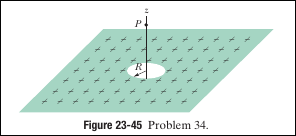
\includegraphics[scale=0.75]{image-5.png}
\end{figure}

\subsection*{Solution}
The electric field of the infinite plane is given by;
\begin{align*}
    E &= \frac{\sigma}{2\varepsilon_0}
\end{align*}
and the electric field from a disc is given by;
\begin{align*}
    E &= \frac{\sigma}{2\varepsilon_0}\left(1 - \frac{z}{\sqrt{z^2 + R^2}}\right)
\end{align*}
which is important because we can think of the hole as a superposition of the infinite plane and the disc, meaning that we can add the two fields together to get the net field at the point $P$.
\begin{align*}
    E &= \frac{\sigma}{2\varepsilon_0} - \frac{\sigma}{2\varepsilon_0}\left(1 - \frac{z}{\sqrt{z^2 + R^2}}\right) \\
    &= \frac{z}{\sqrt{z^2 + R^2}}\frac{\sigma}{2\varepsilon_0} \\
    &= \frac{0.0256}{\sqrt{(0.0256)^2 + (0.018)^2}}\cdot\frac{4.5 \times 10^{-12}}{2\left(8.85 \times 10^{-12}\right)} \\
    &= \boxed{0.208 \frac{\N}{\C}}
\end{align*}

% \begin{figure}[ht]
%     \centering
%     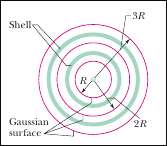
\includegraphics[scale=0.75]{image.png}
% \end{figure}

\end{document}
